% Chapter 1

\chapter{Experiments} % Main chapter title

\label{Chapter8}

In this chapter we display a novel usage to our new the $ID$ method attributes and qualities. Here we will use our $ID$ method in order to obtain a \textbf{perceptual colors distance metric learning} \cite{perp_color}, which is a high demanded function in computer vision region.\\ 
Our examination is based and referring to \cite{perp_color} and \cite{c2lm} papers, which developed a local metric embedding method for this problem. 

This set of experiments models a perceptual color difference metrics, based on various color samples originated from several cameras, angles, illuminations etc.
\\

Our $ID$ method would be examined in this section solely by the original experiment's accuracy measures - Mean Absolute Error \cite{MAE}, along various parameters such number of centers per dimension, and different datasets assembly.
\\
Further discussion will refer to the various exams may apply on our $ID$ method according to our described theory.

\section{Experiment Procedure}

\textbf{object pairs ID embedding} \ref{Chapter3} will be demonstrated by applying its embedding method over pairs which was taken and labeled from the Farnsworth-Munsell 100 hue-test set \cite{farnsworth}.
\subsection{Dataset}

Dataset of this experiment is assembled from single color patches, which displayed in a set of images, where each image was generated by a specific set of image features, such illumination, camera type (4 different cameras are involved in the dataset creation) , lance type , background etc.

\begin{figure}[H] \label{set_ds}
			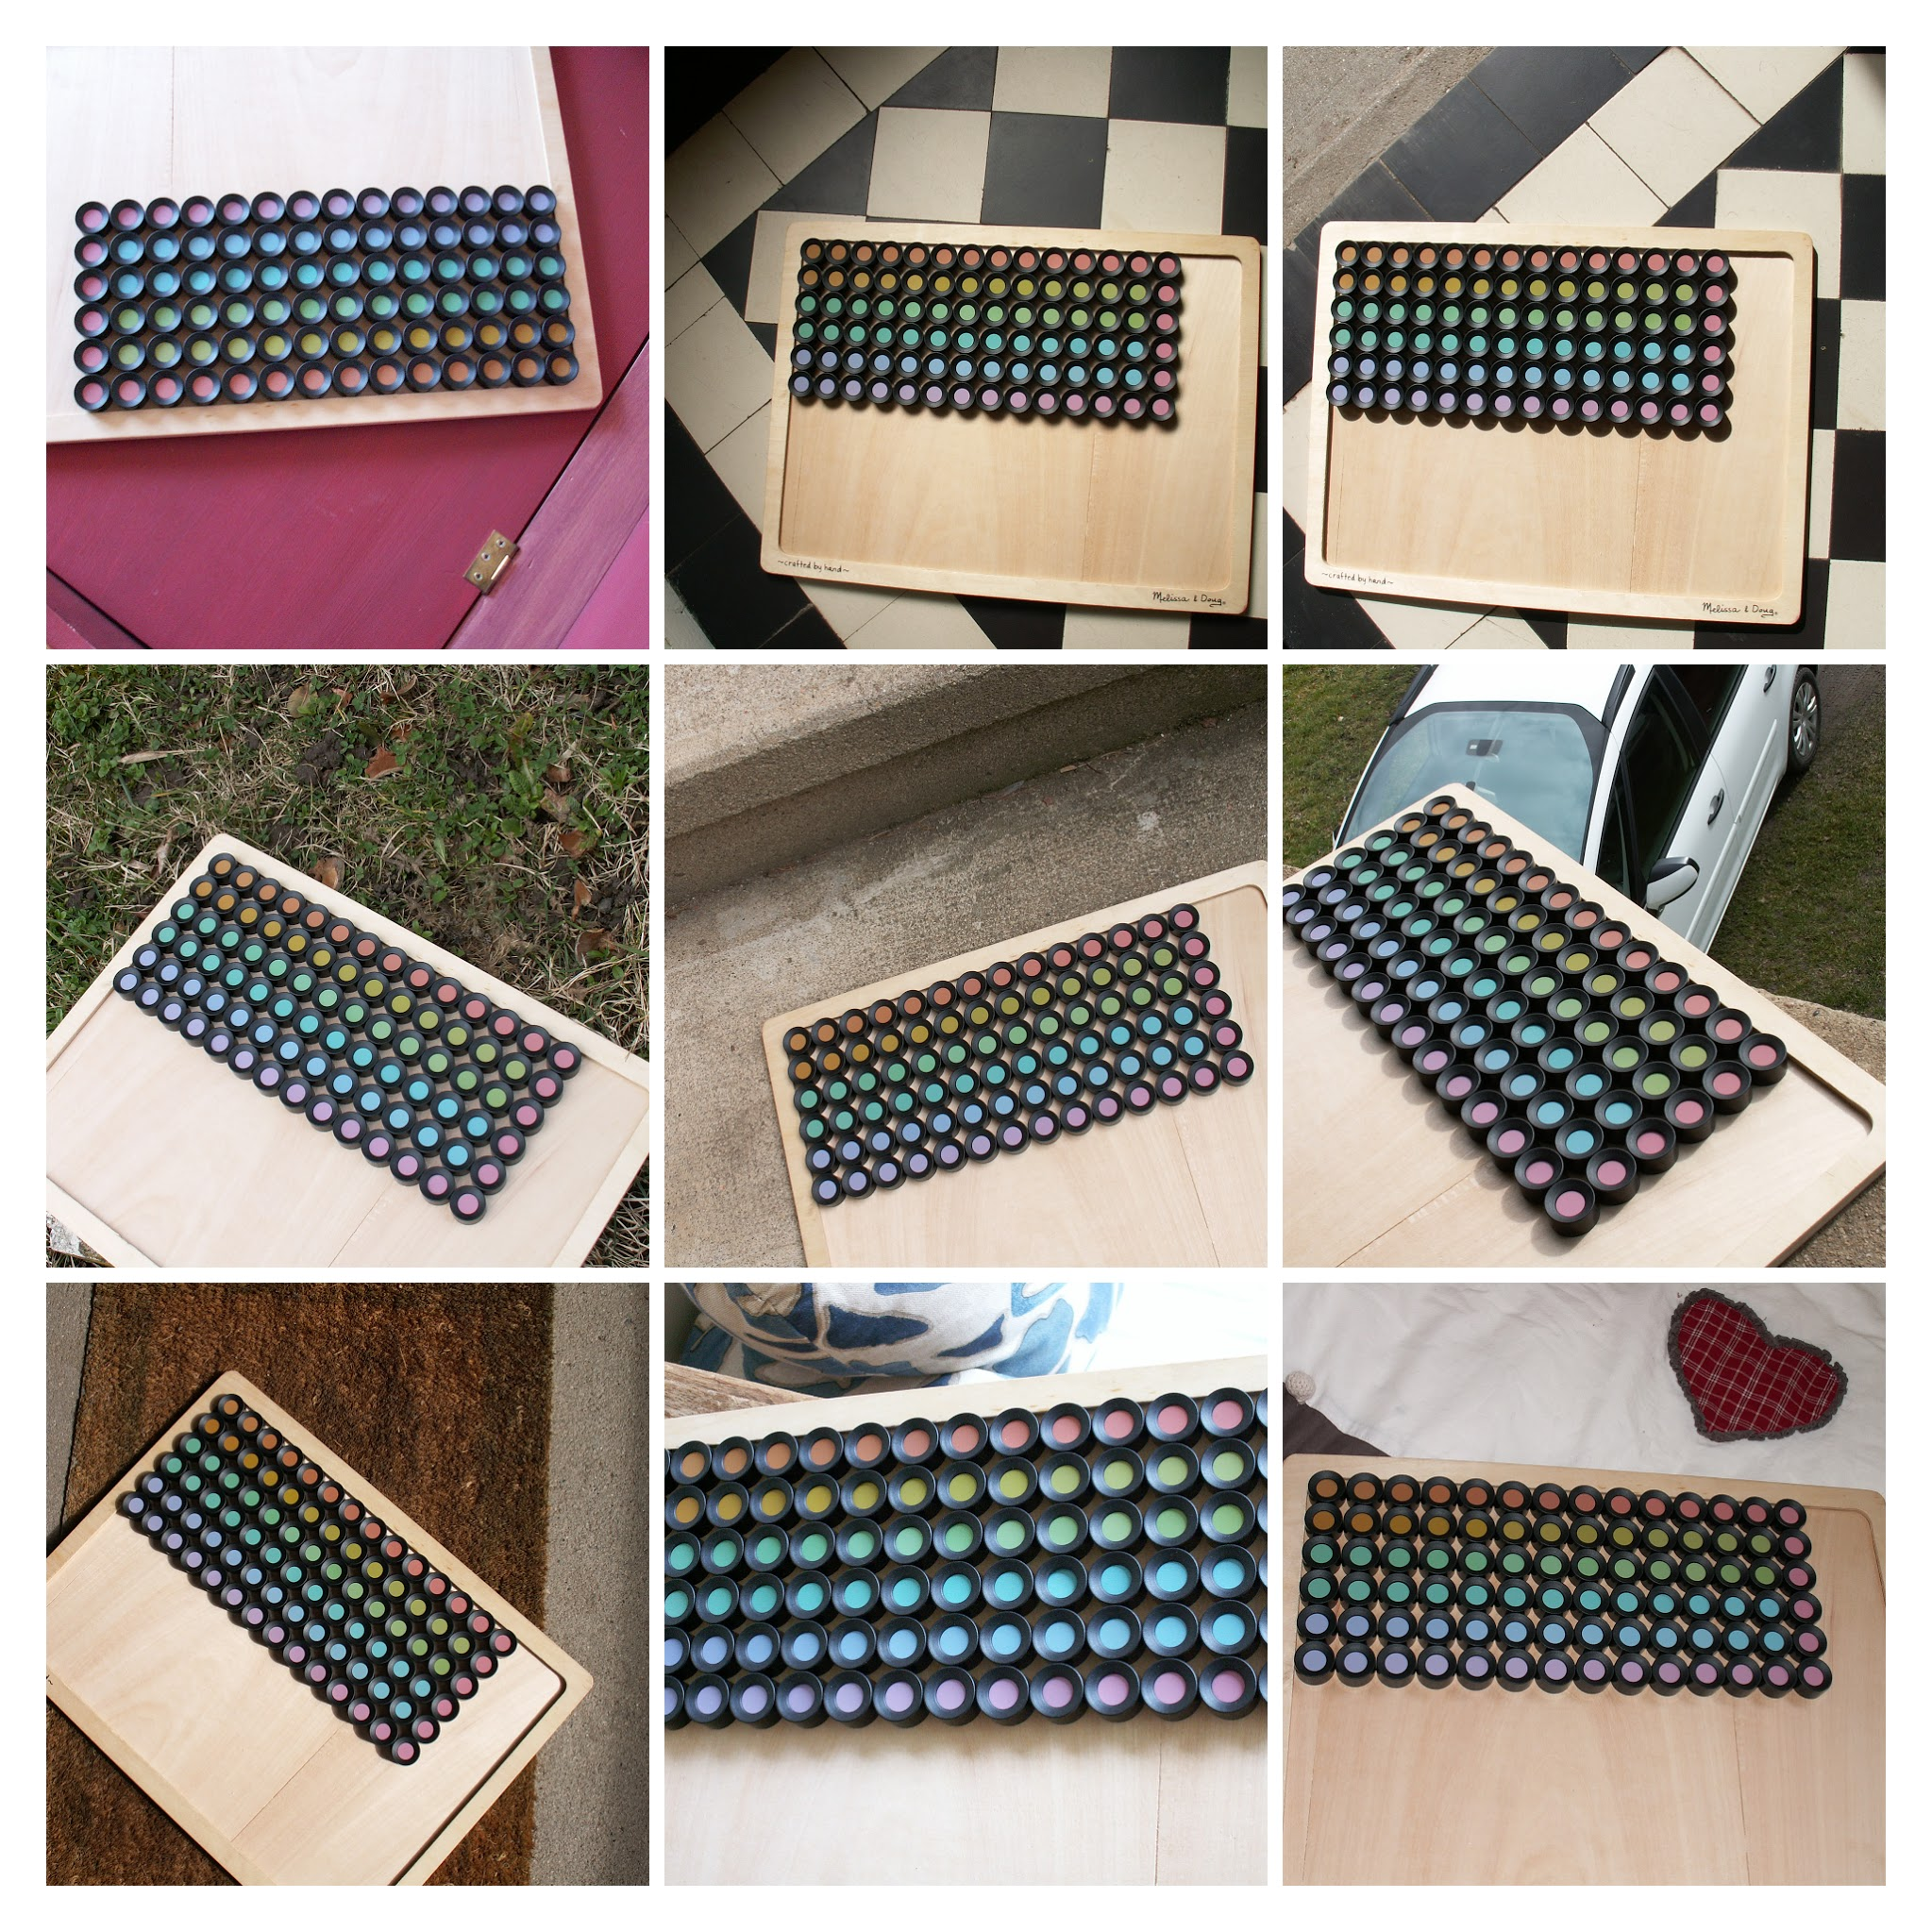
\includegraphics[width=\linewidth,height=12cm,keepaspectratio]{Figures/set_ds}
			\caption[set ds]
			{dataset patches original images formats}
\end{figure}

For each color patch, a $L^*A^*B^*$ \cite{lab} coordinates are given. 
Since the pairs of patches should be close by their CIELAB \cite{CIELAB} coordinates in order to adapt a good color difference assessment, a set in the final dataset is only a set of patches, where its CIELAB euclidean distance is relatively close, i.e. $\Delta E \leq 5$ .


%\begin{figure}[H] \label{patch_positions}
%			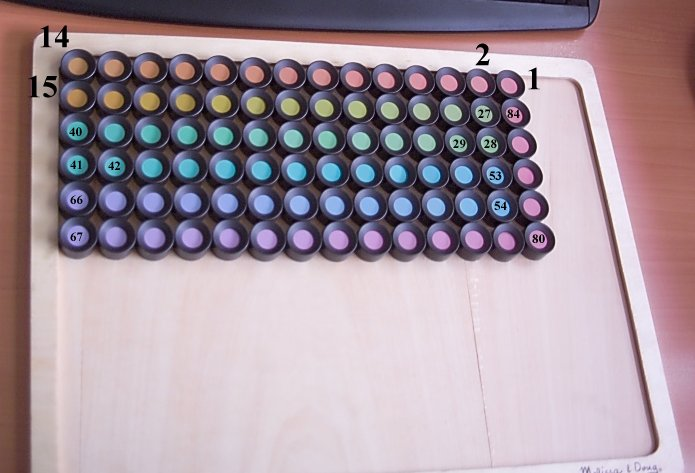
\includegraphics[width=\linewidth,height=12cm,keepaspectratio]{Figures/patch_positions}
%			\caption[color patches order in every samples image]
%			{patches order}
%\end{figure}


\subsection{Models to train}
\label{color_cam}
Then, $ID$ learning method will try to learn some similarity models according to a couple of test conditions:

\begin{itemize}
	\item \textbf{unseen colors} - dividing the entire patches set into train-test sets
	\item \textbf{unseen cameras} - assigning 3 out of 4 cameras sets as train set, and make the remained camera set as test set. \\
		training set cameras:
		\begin{itemize}
			\item Kodak DCS	Pro 14n
			\item Konica Minolta Dimage Z3
			\item Nikon Coolpix S6150
		\end{itemize}	
		
		test set camera:	
		\begin{itemize}
			\item Sony DCR-SR32
		\end{itemize}
		
\end{itemize}

\subsection{Interpolation}
Data dimension in our scenarios is of course $n=3$ (for lab/RGB \cite{RGB} coordinates), and for an object pair the dimension is $2n=6$. \\
As described in \ref{Chapter3}, interpolation is performed dimension-wise along the training set, after selecting data center per dimension by manual or automatic (k-means) method.
\\
In our experiment we have selected cross validation \cite{cross_val} over certain fold number of our dataset for assessing the optimal number of centers per dimension, and find those by using k-means \cite{kmeans} algorithm.





For the selected number of extracted centers we add two extreme points for applying proper interpolation for data values beyond limits of the discovered centers.
\\
Now that we have found data centers for each dimension we apply our interpolation method \ref{Chapter3} on our data (on both train-test sets) and extract a $\overrightarrow{a} \in \Re^3$ coefficient vector per color patches pair, which is ready to be embedded.


\subsection{Embedding}
Our dataset is now embedded by applying an embedding of the coefficient vectors on a sparse form such: 
\vskip5pt
$\overrightarrow{e} \in \Re^{2\prod_{i=1}^{n}{length(\overrightarrow{c_i})}}$ 
\vskip5pt
where $n = 3$.
\vskip5pt
Each coefficient vector element is assigned to the exact simplex index in the $\overrightarrow{e}$ embedded vector.
\\

\subsection{Learning}
Learning phase is performed on a linear regression model training process.
As described on \ref{learn_regression}, we learn by using \textbf{Stochastic Gradient Descent} \cite{SGD} optimization algorithm, regularized by a known distance such $\lone$. \\
Loss function of the training process would be a generalized Mean Average Error \cite{MAE} loss function, constrained by our semi-metrics critireas for model divergence as described in the learning chapter \ref{Chapter5}:
%\begin{equation}
%\wopt & = \\
%& \argmin_{\wadd} 
%\Bigg( 
%\learningregtwo + 
%\\
%& C \sum_{i=1}^{\pairsnum}
%\Big(
%\distreg(\xvpairsindexifirst,\xvpairsindexisecond) + 
%\ope(\xvpairsindexifirst,\xvpairsindexisecond) \cdot \wadd - \\
%& \simlabel_i\Big)^2
%\Bigg)
%\end{equation}


\subsection{Assessment}
Models assessment is applied by following criteria:
\begin{itemize}
\item \textbf{MAE} - Mean Absolute Error
\end{itemize}

The test set of each experiment is processed by our embedding method and a  distance figure is calculated. This figure $y_i^{test}$ is being compared to the predicted label for each sample by assembling the MAE index:
\begin{equation}
MAE = \frac{1}{n} \cdot \sum_{i = 1}^{n}{|y^{pred}_i - y^{test}_i|}
\end{equation}
Where n is test set size. \\


\section{Results}

Let us describe our results being compared to the original paper results as described in \ref{original paper results}.
We display the experiments for each data splitting (camera/color). 
Our experiments performed by applying cross validation algorithm mentioned at  \ref{cross_validation}.
Let us observe the experiments performed on data splits described \ref{color_cam}.
\\

Along all the experiments we perform sweep over the number of centers per dimension $c \in [2,10]$, which will describe the behavior of all models over datasets' dispersion.
\\
We display several examinations of our results:
\begin{itemize}
	\item \textbf{regularizers scan} - $L1, L2, \Delta E$
	\item \textbf{train .vs. test} sets error
	\item \textbf{unseen colors .vs. unseen cameras}	
\end{itemize}
We also describe a comparison of results based centers extracted by cross validation algo.


\subsection{Cross-Validation Centers}

\begin{itemize}
	\item Unseen Colors

Unseen color case was assembled by a certain percentage of all data set as train set, and the rest as test set. In this experiment we have taken the train set size to be $80 \%$ of the total data set.

	\subsubsection{Dataset properties}
	
	From a total 13500 patches pairs set, the divided train-test sets amounts are:
	\begin{table}[H]
		\centering
		\label{test_train1}
		\begin{tabular}{|c|c|}
			\textbf{set} & \textbf{size} \\ \hline \textbf{train} & \textbf{10800} \\ \hline
			\textbf{test} & \textbf{2700} \\ \hline
		\end{tabular}
		\caption{train/set ratio = $4/1$}
	\end{table}
		
	\subsubsection{Centers locations}
	
	Centers locations are shown as extracted via cross-validation \ref{cross_validation} for finding optimal number of centers per dimension, and k-means for extracting centers values. \\
	k-means actually found only the inner centers, since the outer centers are fixed bounds.\\
	
	
	\begin{matrix}  \qquad  c_0 \quad  \qquad c_1 \quad  \qquad c_2 \end{matrix}\\
			
	
	\begin{pmatrix}
\label{key}     0.0 &     0.0 &    0.0\\
				44.5 &   30.35 &    43.13 \\
				84.4 &   80.28 &    83.43 \\
				161.59 &   150.96 &   168.81\\
     		 255.0 &  255.0 &   255.0 \\
	\end{pmatrix}
	
	\vskip10pt


	\subsubsection{Experiment Figures}
	
	Our model provides the following figures:

	\begin{itemize}
	\item 	p-value = $3.9 \cdot 10 ^{-03}$
	\item 	MAE = $0.80$
	
	\end{itemize}


\item Unseen Camera
%\subsection{Unseen Camera}

Unseen camera scenario was assembled by assigning one of the cameras involved in dataset generation as test set, where the other 3 functions as train set.


	\subsubsection{Dataset properties}
	
		From a total 13500 patches pairs set, the divided train-test sets amounts are:
		\begin{itemize}
			\item \textbf{train set size} = $8084$ 
			\item \textbf{test set size} = $5416$ (Sony DCR-SR32 camera set)
		\end{itemize}
		
		\begin{table}[H]
			\centering
			\label{test_train2}
			\begin{tabular}{|c|c|c|}
				\hline
				\textbf{set} & \textbf{size} & \textbf{cameras} \\ \hline \textbf{train} & \textbf{8084} & \textbf{Kodak DCS Pro 14n, Konica Minolta Dimage Z3,
					Nikon Coolpix S6150} \\ \hline
				\textbf{test} & \textbf{5416} & \textbf{Sony DCR-SR32}\\ \hline
			\end{tabular}
			\caption{train/set ratio = $3/2$}
		\end{table}
		

	\subsubsection{Centers locations}
	
	Centers locations are shown as extracted via cross-validation \cite{cross_val}. for finding optimal number of centers per dimension, and k-means for extracting centers values.\\
	k-means actually found only the inner centers, since the outer centers are fixed bounds.

	\vskip30pt
	\begin{matrix}  \qquad  c_0 \quad  \qquad c_1 \quad  \qquad c_2 \end{matrix}
			
	
		\begin{pmatrix}
		0.0 &     0.0 &    0.0\\
		50.6 &   90.55 &    84.43 \\
		101.54 &    &   \\		
		171.29 &   160.98 &   158.21\\
		255.0 &  255.0 &   255.0 \\
	\end{pmatrix}
	\\

	As seen in centers list, edges are equal per dimension $[0.0 , 255.0]$ for data bounding.
	
	\subsubsection{Experiment Figures}	
	Our model provides the following figures:	
	\begin{itemize}
	\item 	p-value = $4.5 \cdot 10 ^{-05}$
	\item 	MAE = $0.79$
	
	\end{itemize}

\end{itemize}


\subsection{Regularizers Comparison}



\subsection{Train/Test sets Comparison}


\subsection{Unseen colors/Unseen camera sets Comparison}





\section{Comparison}

\begin{figure}[H] 
	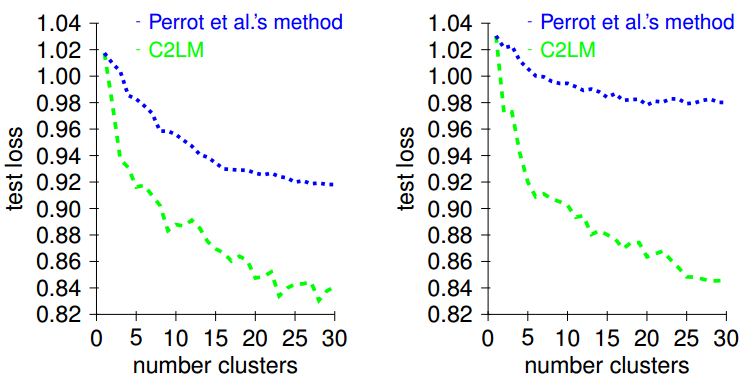
\includegraphics[width=\linewidth,height=10cm,keepaspectratio]{Figures/orig_paper_charts}
	\caption[orig res]
	{original paper test loss charts, as function of cluster numbers}
	\label{original paper results}			
\end{figure}


Let us treat our results versus the original paper's results.\\

While \cite{perp_color} (regression) method
\ref{original paper results} shows results for either camera/color scenarios for model assessment with MAE. \\
The \ref{original paper results} charts' x - axes describes the number of clusters been used in their embedding algorithm. \\
Their minimal values on both scenarios are \textbf{ > 0.82 for MAE}, where our results are \textbf{ < 0.80 for MAE}, all for a $p-value$ with a similar magnitude to theirs. \\
As clearly seen, our results applies the following conditions:
\begin{itemize}
	\item Slight outperforming reference original paper error scores
	\item Small p-values which proves the validity of our method, since there is a reasonable assumption that our models provide close dataset approximation
	\item Overfitting avoidance by applying cross validated centers based on our training set solely.
\end{itemize}

This information is a meaningful confirmation of the assumption that our method is valid to work with in terms of reliability. In the following chapter we will discuss the further explorations should be performed to examine the rest of performance criterias mentioned above.
